\subsection{Review}
\begin{mdframed}[linewidth=1]
\section*{Concept Review}
\textbf{Isomorphisms}: An \emph{isomorphism} is a function which preserves the structure of a model. Formally, an isomorphism from $A$ onto $B$ is a bijection $f$ from $U^A$ to $U^B$ such that $\langle f(i), f(j) \rangle \in L^B \iff \langle i, j \rangle \in L^A$. 

\textbf{Automorphisms}: An \emph{automorphism} an isomorphism from a structure $A$ onto itself; in other words, it is an isomorphism which leaves the edge-set unchanged. $\aut{A}$ is the set of automorphisms of $A$.

%The \emph{automorphism class} of a structure is the set of all functions which are automorphisms on that structure. 

\textbf{Image of a Structure}: The structure $f[A]$, the \emph{image of} $A$ under the function $f$, is the structure with the same universe as $A$ and with the edge relation defined by $L^{f[A]} := \{\langle f(i), f(j) \rangle \mid \langle i, j \rangle \in L^A\}$. 

\textbf{Orbit of a node}: The orbit of a node $a$ in a graph $A$ is the set of all images of that node under automorphisms of the graph. Intuitively, this is the set of all nodes which ``look the same, structurally'' as $a$. 

\textbf{Orbit of a graph}: The orbit of a graph $A\in\modn{\sg}{k}$  under the action of $\symn{k}$ (the permutation group on $[k]$) is the set of all graphs $B\in\modn{\sg}{k}$ such that $A\cong B$.%is the maximal set of pairwise non-automorphic graphs which can be obtained from $A$ by actions in \symn{k}. In other words, this is the maximal set of graphs isomorphic to $A$, all with different edge-sets. 

\textbf{Definability in the Finite}: The definable subsets of a finite graph are exactly the unions of orbits of its nodes. We categorized all size-4 simple graphs and found all of their definable subsets. 

\textbf{Definability in the Infinite}: Every definable subset of an infinite graph is a union of orbits of (some) of its nodes. It is not the case (in general) that every orbit is definable, nor every union thereof, however, so one must give an explicit schema which defines an orbit in order to assert that it is definable. We saw the examples of the integers with absolute-value and the natural numbers with successor. In the former case, we showed that there were $8$ possible definable sets, generated by the three orbits $\{0\}, \mathbb{Z}^{-}, \mathbb{Z}^{+}$. In the latter case, we used the Compactness Theorem to show that the only definable subsets were the finite and cofinite sets. 

\textbf{Orbit-Stabilizer Theorem}: We gave a proof for the Orbit-Stabilizer Theorem, which states that $|\symn{n}| = |\orb{A}{\symn{n}}| \cdot |\aut{A}|$. 
\iffalse
\textbf{Proof}: We motivated the need for a formal system of proof, and showed that the set of finitely-valid sentences was \emph{semi-decidable}. We remarked that the set of valid sentences does not have an obvious semi-decision procedure like finite validity does, but that validity is still semi-decidable (!) because of the coinciding nature of truth and proof: the \emph{soundness} and \emph{completeness} theorems ensure that every valid formula is provable and vice-versa, and so by enumerating proofs we obtain a semi-decision procedure for validity. We remarked that non-validity (or equivalently, satisfiability) is not semi-decidable, because if it were then validity would itself be decidable (contradicting the Church-Turing Theorem). 

We gave examples of various proofs using the system of \emph{natural deduction} explained in Goldfarb.
\fi 
\end{mdframed}



\newpage
\begin{mdframed}[linewidth=1]
\section*{Problems}
\begin{enumerate}
    \item We say that a list $L$ of structures is \emph{succinct} iff no pair of structures on the list are isomorphic. Give a maximal succinct list of $\modn{S}{3}$ where 
    \[
        S := (\forall x)(\exists y)(\forall z)(Lxz \equiv z = y)
    \]

    \item For each structure $A$ in your list $L$ and each $O \in \autorbs{A}$, give a schema $S(x)$ such that $S[A] = O$. 

    \item Let $A$ be the structure with triadic predicate $P$ defined by 
    \[
        U^A = \mathbb{Z}, P^A = \{\langle i, j, k \rangle \mid |i - j| = k\}
    \]
    Is $X = \{i \in \mathbb{Z} \mid i < 0\}$ definable in $A$?

    \item Let $B$ be the structure with triadic predicte $Q$ defined by
    \[
        U^B = \mathbb{Z}, Q^B = \{\langle i, j, k \rangle \mid i + j = k\}
    \]
    Is $X = \{i \in \mathbb{Z} \mid i < 0\}$ definable in $B$?

    \item 
Let $X$ be the conjunction of the following schemata.
\begin{itemize}
\item 
$(\forall x)(\forall y)(\forall z)((Lxy \wedge Lyz) \supset Lxz)$
\item
$(\forall x)(\forall y)(x\neq y\supset(Lxy \vee Lyx))$
\item
$(\forall x) \neg Lxx$
\item 
$(\forall x)(\exists y)(Lxy\wedge (\forall z)\neg (Lxz\wedge Lzy))$
\item 
$(\forall x)(\exists y)(Lyx\wedge (\forall z)\neg (Lyz\wedge Lzx))$
\item
$(\forall x)(\exists y)(Lyx\wedge Fy)$
\item
$(\forall x)(\exists y)(Lxy\wedge Fy)$
\item
$(\forall x)(\forall y)((Fx\wedge Fy\wedge Lxy)\supset (\exists z)(Fz\wedge Lxz\wedge Lzy))$
\end{itemize}

Is $X$ satisfiable?
\iffalse    
    \item Let 
    \[
        X = (\exists y)(\forall x)(Lxy \vee Lyx)
    \]
    \[
        S = (\forall x)(\exists y)(Lxy \vee Lyx)
    \]
    Does $X$ imply $S$? If so, give a deduction. If not, give a counterexample. 
\fi
    \item Let
    \[
        X = (\exists^{=5}x) \land (\forall x)(\lnot Lxx) \land (\forall xy)(Lxy \supset Lyx)
    \]
    \[
        S = (\exists xyz)(Lxy \land Lxz \land Lyz) \vee (\exists xyz)(\lnot Lxy \land \lnot Lxz \land \lnot Lyz\land x\neq y\land x\neq z\land y\neq z)
    \]
    Does $X$ imply $S$? If so, give a deduction. If not, give a counterexample. 

    \item Let $S$ be the schema
    \[
            (\forall x)(Fx\supset(\exists y)(\neg Fy\wedge(\forall z)(Lxz\equiv y=z)))
    \]
    For each $n\geq 2$, let $R_n$ be the schema
    \[
    (\forall y)(\neg Fy\supset(\exists x_1)\ldots(\exists x_n)\bigwedge_{1\leq i<j\leq n}(x_i\neq x_j\wedge Fx_i\wedge Lx_iy));
    \]
    and for each $n\geq 2$, let $T_n$ be the schema
    \[
    (\exists x_1)\ldots(\exists x_n)\bigwedge_{1\leq i<j\leq n}(x_i\neq x_j\wedge \neg Fx_i).
    \]
    Let $X=\{S,R_n,T_n\mid n\geq 2\}$.

    Is $X$ satisfiable?

\end{enumerate}
\end{mdframed}

\newpage
\begin{mdframed}[linewidth=1]
\section*{Solutions}
\begin{enumerate}
    \item $S$ suffices to say that $L$ is a function. Drawing size-3 graphs leads us to the following maximal collection. 


    \begin{center}
    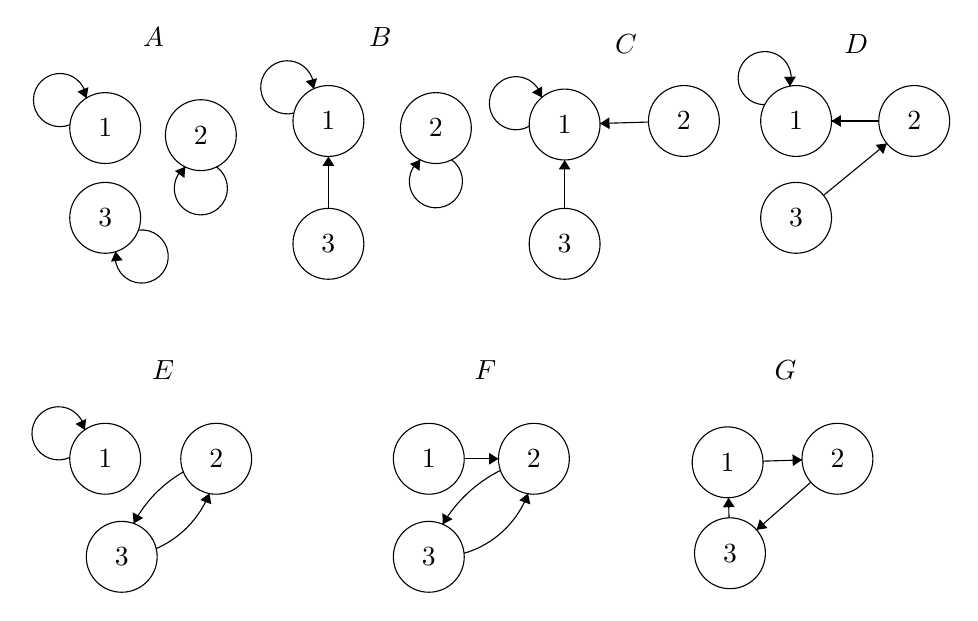
\begin{tikzpicture}[scale=0.15]
    \tikzstyle{every node}+=[inner sep=0pt]
    % \draw [black] (11.4,-11.3) circle (3);
    \draw (11.4,-11.3) node {$A$};
    % \draw [black] (30.6,-11.3) circle (3);
    \draw (30.6,-11.3) node {$B$};
    % \draw [black] (51.4,-11.9) circle (3);
    \draw (51.4,-11.9) node {$C$};
    % \draw [black] (70.9,-11.9) circle (3);
    \draw (70.9,-11.9) node {$D$};
    % \draw [black] (12.2,-39.5) circle (3);
    \draw (12.2,-39.5) node {$E$};
    % \draw [black] (39.5,-39.5) circle (3);
    \draw (39.5,-39.5) node {$F$};
    % \draw [black] (64.9,-39.5) circle (3);
    \draw (64.9,-39.5) node {$G$};
    \draw [black] (7.3,-19) circle (3);
    \draw (7.3,-19) node {$1$};
    \draw [black] (7.3,-26.6) circle (3);
    \draw (7.3,-26.6) node {$3$};
    \draw [black] (15.4,-19.6) circle (3);
    \draw (15.4,-19.6) node {$2$};
    \draw [black] (26.2,-18.4) circle (3);
    \draw (26.2,-18.4) node {$1$};
    \draw [black] (26.2,-28.8) circle (3);
    \draw (26.2,-28.8) node {$3$};
    \draw [black] (35.3,-19) circle (3);
    \draw (35.3,-19) node {$2$};
    \draw [black] (46.2,-18.7) circle (3);
    \draw (46.2,-18.7) node {$1$};
    \draw [black] (46.2,-28.8) circle (3);
    \draw (46.2,-28.8) node {$3$};
    \draw [black] (56.3,-18.4) circle (3);
    \draw (56.3,-18.4) node {$2$};
    \draw [black] (65.8,-18.4) circle (3);
    \draw (65.8,-18.4) node {$1$};
    \draw [black] (65.8,-26.6) circle (3);
    \draw (65.8,-26.6) node {$3$};
    \draw [black] (75.8,-18.4) circle (3);
    \draw (75.8,-18.4) node {$2$};
    \draw [black] (34.7,-47) circle (3);
    \draw (34.7,-47) node {$1$};
    \draw [black] (34.7,-55.3) circle (3);
    \draw (34.7,-55.3) node {$3$};
    \draw [black] (43.6,-47) circle (3);
    \draw (43.6,-47) node {$2$};
    \draw [black] (60,-47.3) circle (3);
    \draw (60,-47.3) node {$1$};
    \draw [black] (60.2,-55) circle (3);
    \draw (60.2,-55) node {$3$};
    \draw [black] (69.3,-47) circle (3);
    \draw (69.3,-47) node {$2$};
    \draw [black] (7.3,-47) circle (3);
    \draw (7.3,-47) node {$1$};
    \draw [black] (8.7,-55.3) circle (3);
    \draw (8.7,-55.3) node {$3$};
    \draw [black] (16.7,-47) circle (3);
    \draw (16.7,-47) node {$2$};
    \draw [black] (4.325,-18.714) arc (292.24052:4.24052:2.25);
    \fill [black] (5.72,-16.47) -- (5.88,-15.54) -- (4.95,-15.91);
    \draw [black] (10.101,-27.64) arc (97.36342:-190.63658:2.25);
    \fill [black] (8.18,-29.46) -- (7.79,-30.31) -- (8.78,-30.19);
    \draw [black] (16.723,-22.28) arc (54:-234:2.25);
    \fill [black] (14.08,-22.28) -- (13.2,-22.63) -- (14.01,-23.22);
    \draw [black] (26.2,-25.8) -- (26.2,-21.4);
    \fill [black] (26.2,-21.4) -- (25.7,-22.2) -- (26.7,-22.2);
    \draw [black] (23.289,-17.727) arc (284.71059:-3.28941:2.25);
    \fill [black] (24.96,-15.68) -- (25.24,-14.78) -- (24.28,-15.03);
    \draw [black] (36.623,-21.68) arc (54:-234:2.25);
    \fill [black] (33.98,-21.68) -- (33.1,-22.03) -- (33.91,-22.62);
    \draw [black] (46.2,-25.8) -- (46.2,-21.7);
    \fill [black] (46.2,-21.7) -- (45.7,-22.5) -- (46.7,-22.5);
    \draw [black] (43.215,-18.838) arc (300.37062:12.37062:2.25);
    \fill [black] (44.28,-16.41) -- (44.3,-15.47) -- (43.44,-15.98);
    \draw [black] (53.3,-18.49) -- (49.2,-18.61);
    \fill [black] (49.2,-18.61) -- (50.01,-19.09) -- (49.98,-18.09);
    \draw [black] (68.12,-24.7) -- (73.48,-20.3);
    \fill [black] (73.48,-20.3) -- (72.54,-20.42) -- (73.18,-21.2);
    \draw [black] (72.8,-18.4) -- (68.8,-18.4);
    \fill [black] (68.8,-18.4) -- (69.6,-18.9) -- (69.6,-17.9);
    \draw [black] (63.149,-17.021) arc (270.25384:-17.74616:2.25);
    \fill [black] (65.28,-15.46) -- (65.78,-14.65) -- (64.78,-14.66);
    \draw [black] (16.12,-49.927) arc (-21.35064:-66.54055:8.469);
    \fill [black] (16.12,-49.93) -- (15.36,-50.49) -- (16.29,-50.85);
    \draw [black] (9.706,-52.484) arc (152.38382:119.72499:10.806);
    \fill [black] (9.71,-52.48) -- (10.52,-52.01) -- (9.63,-51.54);
    \draw [black] (4.314,-46.878) arc (295.38954:7.38954:2.25);
    \fill [black] (5.58,-44.56) -- (5.69,-43.62) -- (4.79,-44.05);
    \draw [black] (43.101,-49.941) arc (-20.09413:-73.90163:8.208);
    \fill [black] (43.1,-49.94) -- (42.36,-50.52) -- (43.3,-50.86);
    \draw [black] (35.876,-52.549) arc (149.54048:116.46376:11.763);
    \fill [black] (35.88,-52.55) -- (36.71,-52.11) -- (35.85,-51.61);
    \draw [black] (37.7,-47) -- (40.6,-47);
    \fill [black] (40.6,-47) -- (39.8,-46.5) -- (39.8,-47.5);
    \draw [black] (67.05,-48.98) -- (62.45,-53.02);
    \fill [black] (62.45,-53.02) -- (63.38,-52.87) -- (62.72,-52.12);
    \draw [black] (60.12,-52) -- (60.08,-50.3);
    \fill [black] (60.08,-50.3) -- (59.6,-51.11) -- (60.6,-51.09);
    \draw [black] (63,-47.2) -- (66.3,-47.1);
    \fill [black] (66.3,-47.1) -- (65.49,-46.62) -- (65.52,-47.62);
    \end{tikzpicture}
    \end{center}

    \item Let $O_1 = \{1\}, O_2 = \{2\}, O_3 = \{3\}, O_4 = \{2, 3\}, O_5 = \{1, 2, 3\}$. Then 
    \begin{itemize}
        \item $\autorbs{A} = \{O_5\}$. This can be defined by the schema $x = x$. 

        \item $\autorbs{B} = \{O_1, O_2, O_3\}$. $O_1$ can be defined by $Lxx \land (\exists y)(Lyx \land y \neq x)$, $O_2$ can be defined by $Lxx \land \lnot (\exists y)(Lyx \land y \neq x)$, and $O_3$ can be defined by $\lnot Lxx$. 

        \item $\autorbs{C} = \{O_1, O_4\}$. $O_1$ can be defined by $Lxx$, and $O_4$ can be defined by $\lnot Lxx$. 

        \item $\autorbs{D} = \{O_1, O_2, O_3\}$. $O_1$ can be defined by $Lxx$, $O_2$ can be defined by $(\exists y)(Lyx \land x \neq y)$, and $O_3$ can be defined by $\lnot (\exists y)Lyx$. 

        \item $\autorbs{E} = \{O_1, O_4\}$. $O_1$ can be defined by $Lxx$, and $O_4$ can be defined by $\lnot Lxx$. 

        \item $\autorbs{F} = \{O_1, O_2, O_3\}$. $O_1$ can be defined by $\lnot (\exists y)Lyx$, $O_2$ can be defined by $(\exists yz)(Lyx \land Lxz \land z \neq y)$, and $O_3$ can be defined by $(\exists y)(\forall z)(Lzx \equiv y = z)$. 

        \item $\autorbs{G} = \{O_5\}$. This can be defined by the schema $x = x$. 
    \end{itemize}

    \item Yes, it is definable. $P^A$ is the \emph{distance relation}; $\langle i, j, k \rangle \in P^A$ iff the distance between $i, j$ is $k$. No two numbers have a negative distance, so we can define the set of all negative numbers by the schema
    \[
        (\forall yz)(\lnot Pyzx)
    \]

    \item No, it is not definable. The function $h$ defined by $h(i) = -i$ is an automorphism of $B$, but $h[X] \neq X$. 
\iffalse
    \item Yes, $X$ does imply $S$. Here is a derivation
    \[
\begin{array}{lll}
\{1\}   & (1)\ (\exists y)(\forall x)(Lxy \vee Lyx)  & \mathrm{P}\\
\{1, 2\} & (2)\ (\forall x)(Lxy \vee Lyx) & (1)y\ \mathrm{EII}\\
\{1, 2\} & (3)\ (Lxy \vee Lyx) & (2)\ \mathrm{UI}\\
\{1, 2\} & (4)\ (\exists y)(Lxy \vee Lyx) & (3)\ \mathrm{EG}\\
\{1\} & (5)\ (\exists y)(Lxy \vee Lyx) & (4)\{2\}\ \mathrm{EIE}\\
\{1\} & (6)\ (\forall x)(\exists y)(Lxy \vee Lyx) & (5)\ \mathrm{UG}
\end{array}
\]
\fi
    \item $X$ does not imply $S$. $X$ states that we have a simple graph of size 5, and $S$ expresses the \emph{three-mutuality} that we considered on day 1 of class. We shows that a ``friendship pentagon'' lacked 3-mutuality; that same pentagon acts as a counterexample here. 

    \item Yes, it is. To show this, we give a satisfying model for $X$. Recall that $\mathbb{Z}$ is the set of integers and $\mathbb{Q}^+$ is the set of positive rational numbers. Let $A$ be defined by
    \begin{itemize}
    \item
    $U^A= \mathbb{Q}^+\times\mathbb{Z}=\{\op{r}{i}\mid r\in\mathbb{Q}^+\mbox{ and}\ i\in \mathbb{Z}\}$ (the cartesian product of $\mathbb{Q}^+$ and $\mathbb{Z}$).
    \item
    $L^A=\{\op{\op{r}{i}}{\op{s}{j}}\mid r<s\}\cup\{\op{\op{r}{i}}{\op{s}{j}}\mid r=s\mbox{ and }i<j\}$.
    \end{itemize}

    Then $A \models X$. 

    \item Yes, it is. We show that $X$ is satisfiable by constructing a structure $B$ with $B\models X$. $B$ is defined by
    \begin{itemize}
    \item
    $U^B= \mathbb{Z}^+$.
    \item
    $F^B=\{2i\mid i\in\mathbb{Z}^+\}$.
    \item
    $L^B = \{\op{2^i\cdot j}{j}\mid i\in\mathbb{Z}^+\mbox{ and } j\not\in F^B\}$.
    \end{itemize}

\end{enumerate}
\end{mdframed}